After having explored linear techniques in fair detail, we will now take a glance at non-linear dimensionality reduction techniques and get an idea of their applications.

\begin{wrapfigure}[13]{r}{0.5\textwidth}
	\centering
	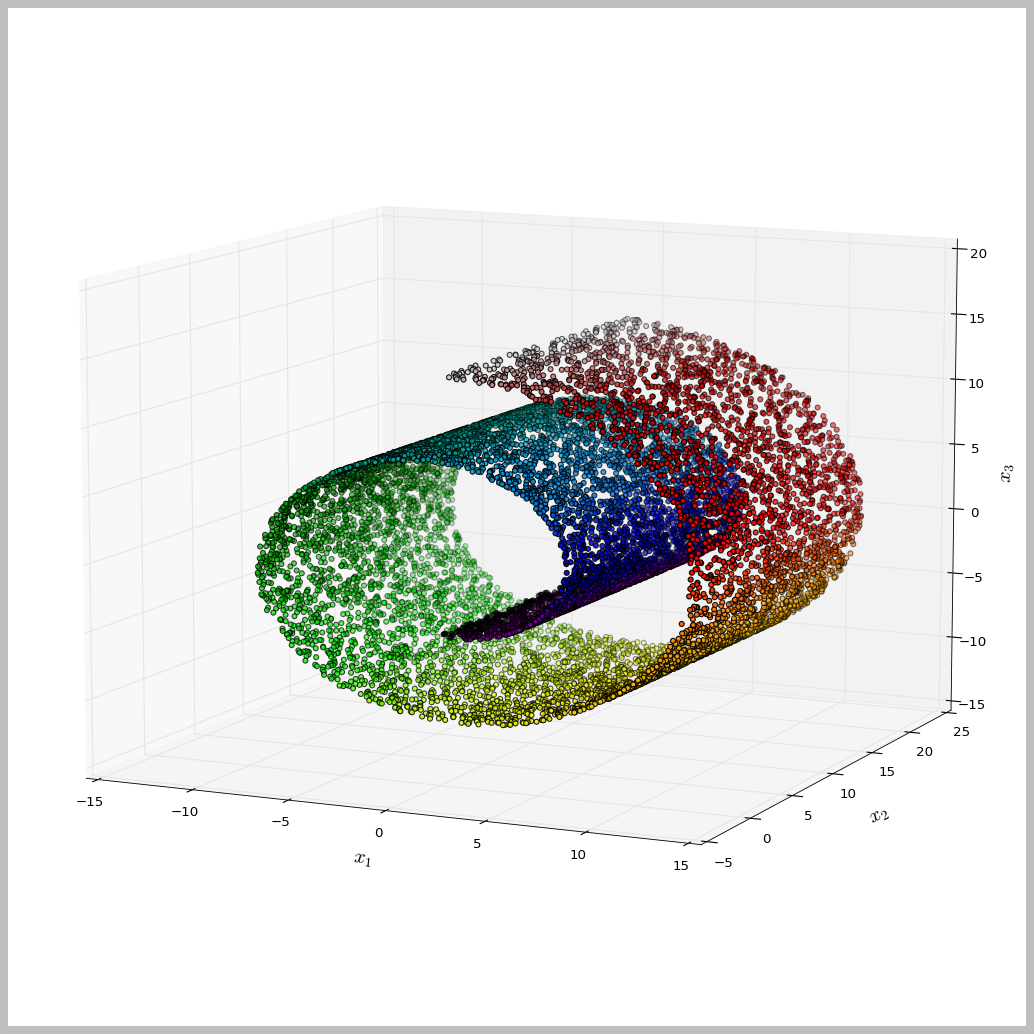
\includegraphics[width=0.4\textwidth]{external_content/graphs/swiss_roll.png}
	\captionsetup{justification=centering}
	\captionof{figure}{Swiss Roll generated from\\ \gls{scikit} \cite{scikit-learn}}
	\label{fig:swissrollfull}
\end{wrapfigure}

In this demonstration, we will look at isomap embedding (often referred as isomap).
First, we will get familiar with the problem domain and then establish a rudimentary theoretical foundation.
Following this, since isomap is primarily used for visualisation \cite{HandsOnMLCh8}, its application is best explained from visual examples.
For this, we will utilise the popular toy example of a swiss roll data set as depicted in adjoining figure \ref{fig:swissrollfull}.

As we can imagine when looking at the swiss roll, a projection of the data or the reduction to a \gls{singular} plane would merely yield insignificant results such as observed in figure \ref{fig:swissrollprojection}.

\begin{wrapfigure}[7]{l}{0.5\textwidth}
	\centering
	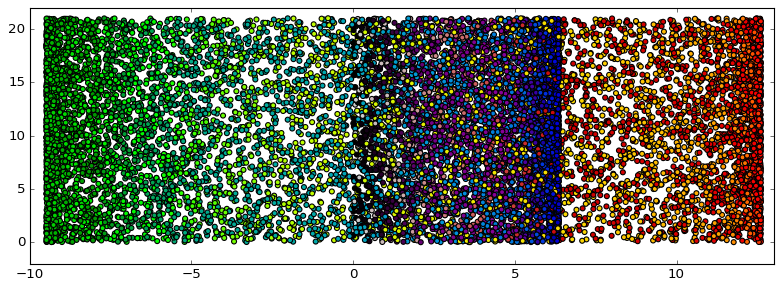
\includegraphics[width=0.38\textwidth]{external_content/graphs/swiss_roll-projection.png}
	\captionsetup{justification=centering}
	\captionof{figure}{Representation in 2D\\ of a projected swiss role}
	\label{fig:swissrollprojection}
\end{wrapfigure}

\vspace{-2mm}
\noindent When faced with this kind of problem, manifold learning should be taken into consideration.
It is an approach to non-linear dimensionality reduction and based on the idea that dimensionality of many data sets is only artificially high.
Manifold learning can be thought of as an attempt to generalise existing linear frameworks to be sensitive to non-linear structures \cite{scikit-learn}.
The isomap embedding algorithm is one of the earliest approaches to manifold learning and has been proposed by \mycite{tenenbaum2000global}.

\begin{wrapfigure}[7]{r}{0.5\textwidth}
	\centering
	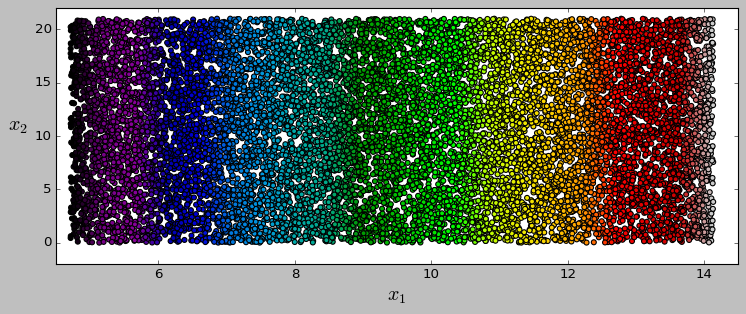
\includegraphics[width=0.45\textwidth]{external_content/graphs/swiss_roll-manifold.png}
	\captionsetup{justification=centering}
	\captionof{figure}{Unrolled swiss roll\\with isomap embedding}
	\label{fig:swissrollmanifold}
\end{wrapfigure}

\noindent
The result and its benefits and be observed in figure \ref{fig:swissrollmanifold}.
Quickly summed up, isomap works in three stages \cite{scikit-learn}:

\begin{enumerate}
	\vspace{-2mm}
	\item Nearest neighbour search
	\vspace{-2mm}
	\item Shortest-path graph search
	\vspace{-2mm}
	\item Partial eigenvalue decomposition
\end{enumerate}


% Significant breakthroughs \cite{ma2012manifold} in this field were accomplished in the year 2000 in the significant and commonly cited paper \emph{A global geometric framework for nonlinear dimensionality reduction}. \cite{tenenbaum2000global}
% To understand the basic idea, we will demonstrate its behaviour to get an idea of the problem using the popular swiss roll data set pictured in figure \ref{fig:swissrollfull}.


% \begin{itemize}
% 	\item First mentioned by \cite{van2008visualizing}
% \end{itemize}

% \clearpage
